% ============================================================================================================
\chapter{Première optimisation des politiques publiques}\label{ch:optimisation}
% ============================================================================================================

\begin{hypothese}[Statut de ce chapitre]
Il ne s'agit pas d'un programme recommandé. L'optimisation sert à identifier les leviers les plus efficaces, les
arbitrages, les interactions entre mesures, et les résultats qui dépendent trop d'hypothèses incertaines. Les
programmes « optimaux » trouvés ici sont optimaux \emph{dans le modèle}, sous ses hypothèses et ses limites
(chapitre~\ref{ch:limites}), et pour les objectifs et contraintes explicitement posés.
\end{hypothese}

\section{Méthode}

\paragraph{Feuille blanche.} L'optimisation part de 35 leviers (tableau~\ref{tab:efficacite}), sans référence aux
programmes A, B, C, D et R de la v0.6, qui ne servent que de points de comparaison (chapitre~\ref{ch:strategies}).
Chaque levier a des bornes plausibles, une difficulté de mise en œuvre (1 à 3) et un niveau de preuve :
\begin{itemize}
\item \textbf{A} : instruments fiscaux et budgétaires, dont les effets passent par les équations estimées et la
microsimulation ;
\item \textbf{B} : réformes structurelles dont l'effet repose sur un comportement documenté par la littérature (âge
légal, assurance chômage, IS, SMIC) ;
\item \textbf{C} : leviers exploratoires ou dont la réalisation est supposée (relocalisation industrielle, R\&D,
formation, droits de douane) ou dont l'effet de long terme repose sur une hypothèse non estimée (durée du travail).
\end{itemize}
Le périmètre principal comprend les leviers A et B ; les leviers C sont ajoutés dans une variante, pour mesurer ce
qu'ils apportent \emph{si} leurs hypothèses sont justes.

\paragraph{Métamodèle.} Chaque levier a été simulé seul avec le modèle complet (68 simulations). La réponse est mise à
l'échelle linéairement ; pour les leviers asymétriques (TVA, IS, cotisations, RSA, investissement public, âge légal,
durée du travail), la hausse et la baisse ont des réponses distinctes. Cette approximation additive est vérifiée a
posteriori : chaque stratégie retenue est resimulée avec le modèle complet (chapitre~\ref{ch:strategies}).

\paragraph{Critères.} Huit critères, mesurés en écart à la référence en 2037 (et à 5, 15 et 20 ans pour la
vérification) : PIB en volume, chômage, dette publique, revenu disponible réel, niveau de vie des 30 \% les plus
modestes, indice de Gini, productivité par emploi, part de l'industrie. Sept indicateurs complémentaires sont publiés
sans être optimisés : solde public, investissement, charge d'intérêts, salaire réel, exportations, emploi, pauvreté,
niveau de vie médian. Le PIB par habitant évolue comme le PIB (la population est la même dans tous les scénarios).

\paragraph{Algorithmes.}
\begin{itemize}
\item \textbf{Front de Pareto} : méthode de l'$\varepsilon$-contrainte (pour chaque niveau d'un critère, meilleur
niveau possible de l'autre) résolue en programme linéaire en nombres mixtes (HiGHS, via SciPy), avec au plus
8 leviers actifs et au plus 1 \% de perte de niveau de vie pour chaque décile ; nuage de 40 000 portefeuilles
aléatoires (3 à 12 leviers) pour visualiser les solutions dominées.
\item \textbf{Stratégies} : chacune maximise un objectif explicite sous contraintes explicites ; une variable binaire
par sens de chaque levier interdit d'utiliser un levier dans les deux sens.
\item \textbf{Optimisation globale sans pondération} : maximisation du minimum des huit critères normalisés (point de
Tchebychev), la normalisation étant l'étendue interquantile de chaque critère sur les portefeuilles aléatoires.
\item \textbf{Robustesse aux préférences} : 300 jeux de poids tirés uniformément sur le simplexe des huit critères,
chacun résolu sous la contrainte de ne pas accroître la dette à 10 ans.
\end{itemize}

\section{Efficacité des leviers pris isolément}

Le tableau~\ref{tab:efficacite} donne l'effet de chaque levier poussé à sa borne. Plusieurs constats se dégagent.
\begin{enumerate}
\item \textbf{Les leviers de consolidation les moins coûteux pour l'activité} sont ceux qui touchent peu la demande
des ménages modestes : droits de succession, impôts de production, IS (au prix d'un peu d'investissement), impôt
sur la fortune, PFU. Dans le modèle, ils réduisent la dette de 1 à 3,7 points en 2037 avec un effet quasi nul sur le
PIB. Leurs effets sur les ménages ne sont pas visibles dans la microsimulation statique (héritiers, actionnaires,
détenteurs de patrimoine) : leur innocuité apparente est en partie un angle mort du modèle.
\item \textbf{Les leviers d'offre} (âge légal, durée du travail, relocalisation, investissement public) ont les effets
les plus grands sur le PIB, de signes opposés sur la dette selon qu'ils sont financés ou non.
\item \textbf{La prime d'activité est presque autofinancée} dans le modèle : +50 \% coûterait 0,2 point de dette en
2037, parce qu'elle augmente la population active de 200 000 personnes. Ce résultat dépend entièrement de
l'élasticité de participation : avec l'élasticité basse, le coût est deux à trois fois plus élevé.
\item \textbf{Les fonctions de dépense ne sont pas différenciées} : 10\md\ de santé, d'éducation ou de fonctionnement
ont le même effet macroéconomique. Le modèle ne mesure pas la qualité des services publics.
\end{enumerate}

{\scriptsize\setlength{\tabcolsep}{3pt}\begin{longtable}{p{4.2cm}rcrrrrr}\caption{Effet de chaque levier poussé à sa borne, seul (modèle complet, comportements centraux, écart à la référence en 2037 ; niveau de vie des 30 \% les plus modestes et Gini : microsimulation statique).}\label{tab:efficacite}\\ \toprule Levier & Valeur & Niv. & PIB (\%) & Chômage (pt) & Dette (pt) & Modestes (\%) & Gini (×100)\\ \midrule\endfirsthead \toprule Levier & Valeur & Niv. & PIB & Chômage & Dette & Modestes & Gini\\ \midrule\endhead
IR 1re tranche (pt) & $+2{,}0$ & A & $-0{,}22$ & $+0{,}18$ & $-1{,}0$ & $-0{,}07$ & $-0{,}09$\\
IR 1re tranche (pt) & $-2{,}0$ & A & $+0{,}22$ & $-0{,}18$ & $+1{,}0$ & $+0{,}07$ & $+0{,}09$\\
IR tranche sup. (pt) & $+10{,}0$ & A & $-0{,}00$ & $+0{,}00$ & $-0{,}1$ & $-0{,}31$ & $-0{,}07$\\
IR tranche sup. (pt) & $-5{,}0$ & A & $+0{,}00$ & $-0{,}00$ & $+0{,}0$ & $+0{,}16$ & $+0{,}03$\\
CSG activité (pt) & $+1{,}5$ & A & $-0{,}40$ & $+0{,}31$ & $-1{,}8$ & $-1{,}03$ & $-0{,}03$\\
CSG activité (pt) & $-1{,}5$ & A & $+0{,}39$ & $-0{,}31$ & $+1{,}2$ & $+1{,}03$ & $+0{,}03$\\
TVA normale (pt) & $+2{,}5$ & A & $-0{,}13$ & $+0{,}26$ & $-4{,}4$ & $-1{,}83$ & $+0{,}07$\\
TVA normale (pt) & $-2{,}0$ & A & $+0{,}03$ & $-0{,}11$ & $+4{,}8$ & $+0{,}77$ & $-0{,}03$\\
TVA réduite (pt) & $+2{,}0$ & A & $-0{,}03$ & $+0{,}08$ & $-2{,}9$ & $-0{,}48$ & $+0{,}03$\\
TVA réduite (pt) & $-2{,}0$ & A & $+0{,}00$ & $-0{,}04$ & $+3{,}4$ & $+0{,}24$ & $-0{,}01$\\
Impôt fortune (\%) & $+1{,}0$ & A & $-0{,}02$ & $+0{,}05$ & $-1{,}1$ & $+0{,}00$ & $-0{,}28$\\
PFU (pt) & $+10{,}0$ & A & $-0{,}02$ & $+0{,}03$ & $-0{,}8$ & $+0{,}00$ & $-0{,}19$\\
PFU (pt) & $-4{,}0$ & A & $+0{,}01$ & $-0{,}01$ & $+0{,}3$ & $-0{,}00$ & $+0{,}08$\\
IS (pt) & $+4{,}7$ & B & $-0{,}37$ & $+0{,}10$ & $-3{,}6$ & $+0{,}00$ & $+0{,}00$\\
IS (pt) & $-5{,}8$ & B & $+0{,}44$ & $-0{,}12$ & $+4{,}7$ & $+0{,}00$ & $+0{,}00$\\
Impôts production (Md€) & $+5{,}0$ & A & $+0{,}01$ & $-0{,}01$ & $-2{,}2$ & $+0{,}00$ & $+0{,}00$\\
Impôts production (Md€) & $-15{,}0$ & A & $-0{,}03$ & $+0{,}03$ & $+6{,}5$ & $-0{,}00$ & $-0{,}00$\\
Cotis. employeurs (Md€) & $+10{,}0$ & A & $-0{,}08$ & $+0{,}19$ & $-2{,}0$ & $+0{,}00$ & $+0{,}00$\\
Cotis. employeurs (Md€) & $-20{,}0$ & A & $+0{,}16$ & $-0{,}36$ & $+3{,}1$ & $+0{,}00$ & $+0{,}00$\\
Successions (\%) & $+50{,}0$ & A & $+0{,}02$ & $-0{,}01$ & $-3{,}3$ & $+0{,}00$ & $+0{,}00$\\
Successions (\%) & $-30{,}0$ & A & $-0{,}01$ & $+0{,}01$ & $+2{,}0$ & $-0{,}00$ & $-0{,}00$\\
Taxe carbone (€/t) & $+100{,}0$ & A & $-0{,}15$ & $+0{,}30$ & $-3{,}0$ & $-2{,}22$ & $+0{,}19$\\
SMIC (\%) & $+8{,}0$ & B & $-0{,}02$ & $+0{,}06$ & $+0{,}5$ & $+0{,}00$ & $+0{,}00$\\
Point d'indice (\%) & $+5{,}0$ & A & $+0{,}17$ & $-0{,}29$ & $+2{,}0$ & $+0{,}00$ & $+0{,}00$\\
Point d'indice (\%) & $-2{,}0$ & A & $-0{,}07$ & $+0{,}12$ & $-0{,}8$ & $-0{,}00$ & $-0{,}00$\\
Emplois publics (k) & $+100{,}0$ & A & $+0{,}10$ & $-0{,}16$ & $-0{,}3$ & $-0{,}00$ & $-0{,}00$\\
Emplois publics (k) & $-170{,}0$ & A & $-0{,}16$ & $+0{,}27$ & $+0{,}5$ & $+0{,}00$ & $+0{,}00$\\
Fonctionnement (Md€) & $+10{,}0$ & A & $+0{,}13$ & $-0{,}24$ & $-0{,}4$ & $-0{,}00$ & $-0{,}00$\\
Fonctionnement (Md€) & $-20{,}0$ & A & $-0{,}25$ & $+0{,}49$ & $+0{,}8$ & $+0{,}00$ & $+0{,}00$\\
Santé (Md€) & $+10{,}0$ & A & $+0{,}13$ & $-0{,}24$ & $-0{,}4$ & $-0{,}00$ & $-0{,}00$\\
Santé (Md€) & $-10{,}0$ & A & $-0{,}13$ & $+0{,}24$ & $+0{,}4$ & $+0{,}00$ & $+0{,}00$\\
Éducation (Md€) & $+10{,}0$ & A & $+0{,}13$ & $-0{,}24$ & $-0{,}4$ & $-0{,}00$ & $-0{,}00$\\
Éducation (Md€) & $-10{,}0$ & A & $-0{,}13$ & $+0{,}24$ & $+0{,}4$ & $+0{,}00$ & $+0{,}00$\\
Défense (Md€) & $+15{,}0$ & A & $+0{,}19$ & $-0{,}37$ & $-0{,}6$ & $-0{,}00$ & $-0{,}00$\\
Défense (Md€) & $-5{,}0$ & A & $-0{,}06$ & $+0{,}12$ & $+0{,}2$ & $+0{,}00$ & $+0{,}00$\\
Invest. public (Md€) & $+30{,}0$ & A & $+1{,}37$ & $-0{,}48$ & $+5{,}8$ & $+0{,}00$ & $+0{,}00$\\
Invest. public (Md€) & $-10{,}0$ & A & $-0{,}46$ & $+0{,}17$ & $-2{,}1$ & $+0{,}00$ & $+0{,}00$\\
Indexation pensions (pt/an) & $+0{,}5$ & A & $+0{,}06$ & $-0{,}12$ & $+1{,}0$ & $+0{,}25$ & $-0{,}03$\\
Indexation pensions (pt/an) & $-1{,}0$ & A & $-0{,}13$ & $+0{,}24$ & $-2{,}1$ & $-0{,}50$ & $+0{,}05$\\
Allocations chômage (\%) & $+10{,}0$ & B & $-0{,}02$ & $+0{,}01$ & $+0{,}9$ & $-0{,}00$ & $-0{,}00$\\
Allocations chômage (\%) & $-25{,}0$ & B & $+0{,}06$ & $-0{,}03$ & $-2{,}2$ & $+0{,}00$ & $+0{,}00$\\
Alloc. familiales (\%) & $+25{,}0$ & A & $+0{,}03$ & $-0{,}05$ & $+0{,}2$ & $+0{,}65$ & $-0{,}14$\\
Alloc. familiales (\%) & $-10{,}0$ & A & $-0{,}01$ & $+0{,}02$ & $-0{,}1$ & $-0{,}26$ & $+0{,}05$\\
Aides logement (\%) & $+10{,}0$ & A & $-0{,}28$ & $+0{,}03$ & $+0{,}8$ & $+0{,}89$ & $-0{,}12$\\
Aides logement (\%) & $-10{,}0$ & A & $+0{,}28$ & $-0{,}03$ & $-0{,}8$ & $-0{,}89$ & $+0{,}12$\\
RSA (\%) & $+25{,}0$ & A & $-0{,}09$ & $-0{,}08$ & $+0{,}5$ & $+2{,}78$ & $-0{,}38$\\
RSA (\%) & $-10{,}0$ & A & $+0{,}04$ & $+0{,}03$ & $-0{,}3$ & $-1{,}00$ & $+0{,}14$\\
Prime d'activité (\%) & $+50{,}0$ & A & $+0{,}72$ & $-0{,}44$ & $+0{,}2$ & $+4{,}92$ & $-1{,}10$\\
Prime d'activité (\%) & $-10{,}0$ & A & $-0{,}14$ & $+0{,}09$ & $-0{,}0$ & $-0{,}98$ & $+0{,}22$\\
Minimum vieillesse (\%) & $+25{,}0$ & A & $+0{,}01$ & $-0{,}02$ & $-0{,}0$ & $+0{,}74$ & $-0{,}07$\\
Transferts (pt PIB) & $+0{,}3$ & A & $+0{,}06$ & $-0{,}11$ & $+1{,}2$ & $+0{,}00$ & $+0{,}00$\\
Transferts (pt PIB) & $-0{,}3$ & A & $-0{,}06$ & $+0{,}12$ & $-1{,}5$ & $+0{,}00$ & $+0{,}00$\\
Logements sociaux (k/an) & $+100{,}0$ & A & $+0{,}14$ & $-0{,}21$ & $-1{,}6$ & $+0{,}00$ & $+0{,}00$\\
Relocalisation (\%) & $+20{,}0$ & C & $+1{,}80$ & $-0{,}85$ & $-9{,}4$ & $+0{,}00$ & $+0{,}00$\\
Droits de douane (\%) & $+10{,}0$ & C & $-0{,}15$ & $+0{,}28$ & $-2{,}1$ & $+0{,}00$ & $+0{,}00$\\
Durée du travail (h) & $+2{,}0$ & C & $+2{,}01$ & $-0{,}71$ & $-4{,}5$ & $+0{,}00$ & $+0{,}00$\\
Durée du travail (h) & $-1{,}0$ & C & $-1{,}01$ & $+0{,}39$ & $+1{,}9$ & $+0{,}00$ & $+0{,}00$\\
Âge légal (ans) & $+2{,}0$ & B & $+1{,}77$ & $+0{,}89$ & $-3{,}2$ & $+0{,}00$ & $+0{,}00$\\
Âge légal (ans) & $-2{,}0$ & B & $-2{,}27$ & $-0{,}37$ & $+5{,}2$ & $+0{,}00$ & $+0{,}00$\\
Aide R\&D (Md€) & $+6{,}0$ & C & $+0{,}86$ & $-0{,}21$ & $+1{,}1$ & $+0{,}00$ & $+0{,}00$\\
Formation (Md€) & $+4{,}0$ & C & $+0{,}11$ & $-0{,}17$ & $-0{,}5$ & $+0{,}00$ & $+0{,}00$\\\bottomrule\end{longtable}}

\section{Front de Pareto et solutions dominées}

Parmi 40 000 portefeuilles aléatoires du périmètre principal, 71 \% sont dominés : il existe un autre portefeuille au
moins aussi bon sur les huit critères et meilleur sur l'un d'eux. Avec les leviers exploratoires, la proportion monte
à 92 \% : la relocalisation et la durée du travail, si leurs hypothèses sont justes, dominent beaucoup de
combinaisons. La figure~\ref{fig:pareto} montre deux arbitrages : chômage contre dette, et niveau de vie des
modestes contre dette.

\begin{figure}[htbp]\centering
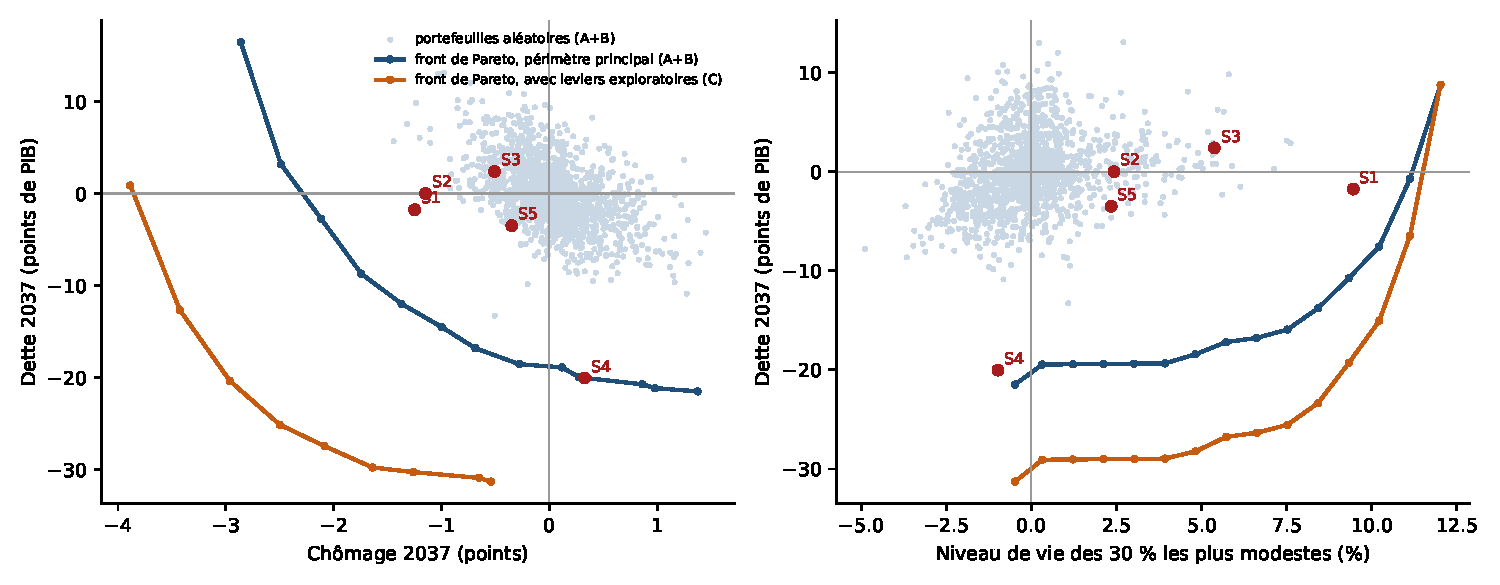
\includegraphics[width=\linewidth]{pareto.pdf}
\caption{Fronts de Pareto à 10 ans (métamodèle, au plus 8 leviers, aucune perte de plus de 1 \% par décile). Points
gris : portefeuilles aléatoires. Points rouges : les cinq stratégies.}\label{fig:pareto}
\end{figure}

\begin{resultat}[Arbitrages (métamodèle, périmètre principal, 8 leviers au plus)]
\begin{itemize}
\item \textbf{Chômage et dette sont conciliables jusqu'à environ deux points de chômage} : le front passe par une
baisse du chômage de 2,1 points avec une dette inférieure de 2,7 points à la référence en 2037 (prime d'activité,
baisse de CSG, dépenses publiques et logements sociaux financés par des économies et des prélèvements). Au-delà,
l'arbitrage devient très coûteux : $-2{,}5$ points de chômage se paient de +3 points de dette, $-2{,}9$ points de
+16 points.
\item \textbf{Désendettement et emploi ne sont pas conciliables au-delà de 15 points} : les portefeuilles qui
réduisent le plus la dette (environ $-21$ points en 2037) augmentent le chômage d'un peu plus d'un point.
\item \textbf{Pouvoir d'achat des modestes et dette sont conciliables sur une large plage} : une hausse de 9 \% du
niveau de vie des 30 \% les plus modestes reste compatible avec une baisse de dette de 10 points, financée par des
prélèvements sur les entreprises, les successions et par l'âge légal ; au-delà de 11 \%, la dette augmente
rapidement.
\item \textbf{Les gains de la variante « exploratoire »} (fronts orange) sont de l'ordre de 10 points de dette
supplémentaires à chômage donné ; ils reposent sur la relocalisation et la durée du travail, dont les effets sont
supposés.
\end{itemize}
Ces fronts sont calculés par le métamodèle additif ; ils surestiment probablement ce qui est atteignable, parce que
les effets de mesures nombreuses et fortes ne s'additionnent pas toujours (vérification au chapitre~\ref{ch:strategies}).
\end{resultat}

\section{Robustesse aux préférences collectives}

Le tableau~\ref{tab:pref} indique, pour 300 jeux de poids tirés au hasard, la proportion des optimums qui utilisent
chaque levier. Il distingue les leviers « robustes aux préférences », retenus quelle que soit la pondération, des
leviers qui dépendent des priorités.

\begin{table}[htbp]\centering\small
\caption{Fréquence d'emploi des leviers dans 300 optimums à poids aléatoires (périmètre principal, dette à 10 ans
non accrue, pertes par décile ≤ 1 \%).}\label{tab:pref}
\tabfit{../tables/preferences.tex}
\end{table}

La hausse de la prime d'activité (97 \% des optimums), du RSA (83 \%), des droits de succession (73 \%), la baisse
de la CSG sur les revenus d'activité (71 \%), le relèvement de l'âge légal (64 \%) et l'investissement public (61 \%)
sont retenus pour presque toutes les préférences. Ce résultat appelle deux réserves : la prime d'activité et le RSA
sont retenus en partie parce qu'ils améliorent plusieurs critères à la fois (pouvoir d'achat, pauvreté, inégalités,
et, pour la prime, emploi) ; les droits de succession parce que leur coût pour les ménages n'est pas mesuré.
